\chapter{Architecture}
\section{Compound Scaling}

The authors proposed a simple yet very effective scaling technique which uses a compound coefficient Phi to uniformly scale network width, depth, and resolution in a principled way:
\begin{figure}[htpb]
\centering
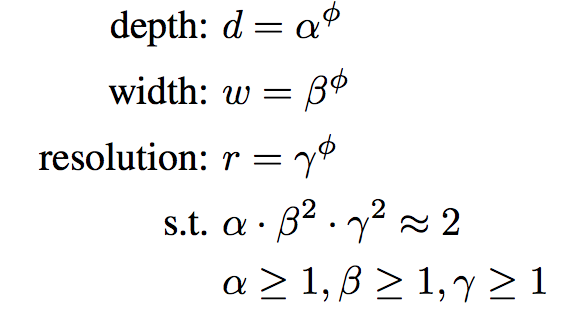
\includegraphics[width=\textwidth,height=\textheight,keepaspectratio]{../../static/Compound Scaling.png}
\caption{Compound Scaling.png}
\end{figure}Phi is a user-specified coefficient that controls how many more resources are available for model scaling. In a CNN, Conv layers are the most compute expensive part of the network. Also, FLOPS of a regular convolution op is almost proportional to d, w squared, r squared, i.e. doubling the depth will double the FLOPS while doubling width or resolution increases FLOPS almost by four times. Hence, in order to make sure that the total FLOPS don’t exceed Phi squared. The constraint applied is that the product of alpha, beta and gamma squared should be nearly equal to 2.
\section{EfficientNet Architecture}

Scaling doesn’t change the layer operations, hence it is better to first have a good baseline network and then scale it along different dimensions using the proposed compound scaling. The authors obtained their base network by doing a Neural Architecture Search (NAS) that optimizes for both accuracy and FLOPS. The architecture is similar to M-NASNet as it has been found using the similar search space. The network layers/blocks are as shown below:
\begin{figure}[htpb]
\centering
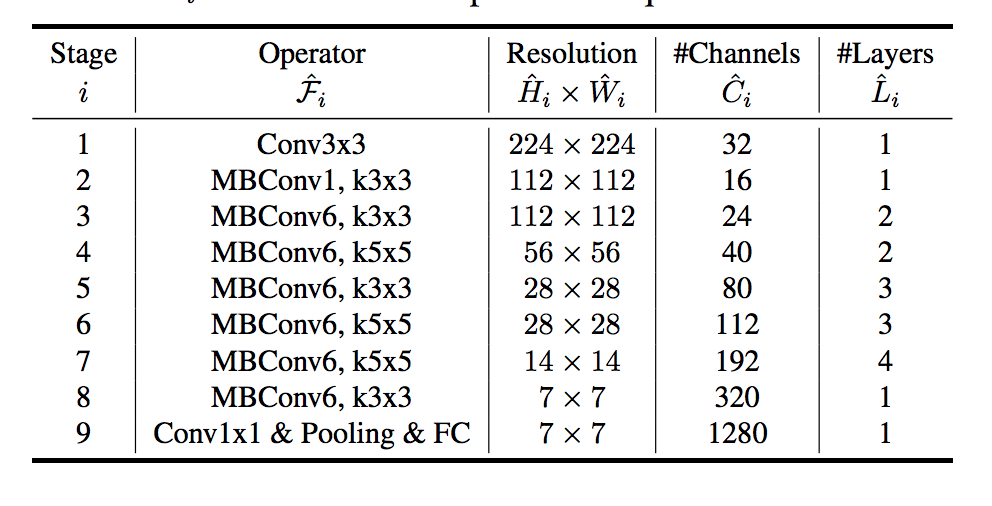
\includegraphics[width=\textwidth,height=\textheight,keepaspectratio]{../../static/EfficientNet baseline network.png}
\caption{EfficientNet baseline network.png}
\end{figure}Now we have the base network, we can search for optimal values for our scaling parameters. If you revisit the equation, you will quickly realize that we have a total of four parameters to search for: alpha, beta, gamma and Phi. In order to make the search space smaller and making the search operation less costly, the search for these parameters can be completed in two steps.

\begin{itemize}
\item Fix Phi as 1, assuming that twice more resources are available, and do a small grid search for alpha, beta and gamma. For baseline network B0, it turned out the optimal values are alpha as 1.2, beta as 1.1, and gamma as 1.15 such that product of alpha, beta and gamma squared is almost equal to 2.
\item Now fix alpha, beta and gamma as constants (with values found in above step) and experiment with different values of Phi. The different values of Phi produce EfficientNets B1-B7.

\end{itemize}